\documentclass{beamer}
%\usetheme{Boadilla}
\usepackage{ru}
\usepackage{amsmath}
%\usepackage{chronosys}
\usepackage{tikz}
\usepackage{epigraph}

\usetikzlibrary{arrows, calc, decorations.markings, positioning}

\input definitions_slides.tex

\title{Church-Turing These}
\subtitle{Een nieuw paradijs}
\author{Pieter van Engelen}
\institute{Radboud Universiteit Nijmegen}
\date{03-06-2022}

\begin{document}

\begin{frame}
    \titlepage
\end{frame}

\begin{frame}
    \tableofcontents
\end{frame}

\section{De tijd}
\begin{frame}
    \begin{timeline}{1925}{1950}{2cm}{2.5cm}{7cm}{10cm}
        \entry{1928}{\small Formulering \emph{Entscheidungsproblem} in \emph{Grundzüge der theoretischen Logik}}
        \entry{1931}{\small Onvolledigheidsstellingen van Gödel}
        \entry{1932}{\small Introductie van de $\lambda$-calculus (A. Church)}
        \entry{1936}{\small Negatieve oplossing \emph{Entscheidungsproblem}}
        \entry{1937}{\small Introductie \emph{turing machine, halting problem} en negatieve oplossing \emph{Entscheidungsproblem}}
        \entry{1939}{\small \emph{Systems of logics based on ordinals} (Turing)}
        \entry{1944}{\small \emph{Introductie Turing-degree} (E. Post)}
        \entry{1945}{\small \emph{First Draft of a Report on the EDVAC} (von Neumann)}
    \end{timeline}    
\end{frame}

\begin{frame}
    \frametitle{De These}
    \begin{center}
        {\Large
            Every \emph{effectively calculable} function is \emph{computable}
        }
        \\
        \bigskip
        \bigskip
        Church (1936), Turing (1937)
    \end{center}
\end{frame}

\subsection{De protagonisten}
\begin{frame}
    \frametitle{De protagonisten}
    \begin{columns}
        \column{0.5\textwidth}
        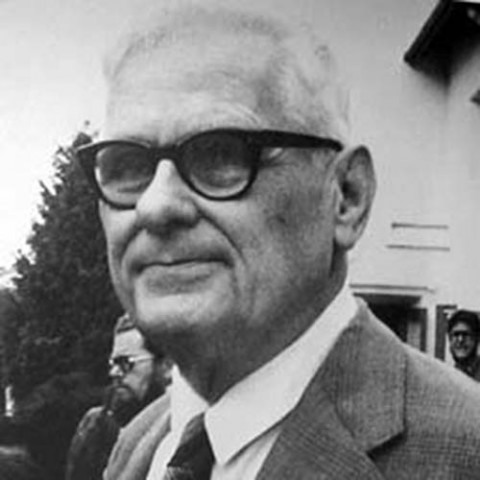
\includegraphics[width=\textwidth]{Church.jpeg}
        \column{0.5\textwidth}
        {\Large Alonzo Church} (1903 - 1995) 

        \emph{Princeton University, USA}
        \begin{itemize}
            \item Logicus, wiskundige
            \item Van 1936 tot 1979 redacteur van \emph{Journal of Symbolic Logic}
            \item 'Bedenker' van de $\lambda$-calculus
            \item Eerste-orde predicaat-logica is onbeslisbaar
            \item Peano-arithmetiek is onbeslisbaar
        \end{itemize}    
    \end{columns}
\end{frame}

\begin{frame}
    \frametitle{De protagonisten}
    \begin{columns}
        \column{0.5\textwidth}
        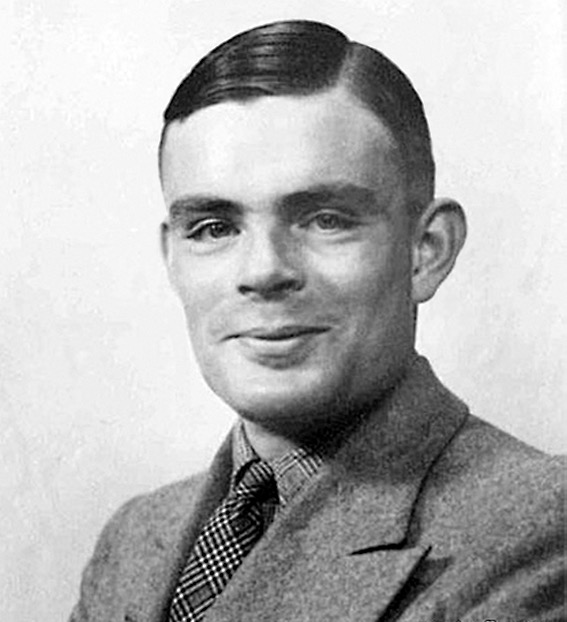
\includegraphics[width=\textwidth]{Turing.jpg}
        \column{0.5\textwidth}
        {\Large Alan Turing} (1912 - 1954) 

        \emph{Cambridge \& Manchester}
        \begin{itemize}
            \item Grondlegger van
            \begin{itemize}
                \item Informatica
                \item Artificiële intelligentie
                \item Morphogenetica
            \end{itemize}
            \item Legendarisch codebreaker
            \item Marathonloper
        \end{itemize}    
    \end{columns}
\end{frame}

\begin{frame}
    \frametitle{De protagonisten}
    \begin{tabular*}{\textwidth}{c c}
        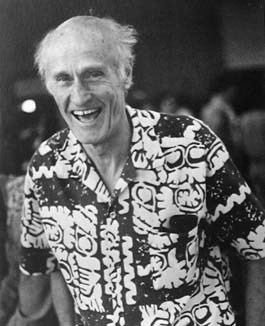
\includegraphics[width=0.4\textwidth]{Kleene.jpeg} & \includegraphics[width=0.4\textwidth]{example-image-duck} \\
        {\large Stephen Kleene} (1909-1994) & {\large ???} (1897 - 1954)\\
    \end{tabular*}
\end{frame}

\section{De situatie}
\subsection{Entscheidungsproblem}
\begin{frame}
    \frametitle{Das Entscheidungsproblem}
    {\large \textbf{Das Entscheidungsproblem}}

    \begin{center}
        Vind een algoritme waarmee \\ 
        de waarheid van een uitspraak in de eerste orde predikaatlogica \\
        vast te stellen is.
        \\
        \bigskip
        {\small \emph{(D. Hilbert \& W. Ackermann, 1928, Grundzüge der theoretischen Logik)}}
    \end{center}
\end{frame}

\begin{frame}
    \frametitle{Entscheidungsproblem}
    \textbf{Eerste orde predikaatlogica} \\
    (extreem kort door de bocht) 
    \bigskip
    
    Logica met
    \begin{itemize}
        \item variabelen
        \item de gebruikelijke operatoren $\wedge, \vee, \rightarrow, \neg, \ldots$
        \item predikaten $P(x)$
        \item universele en existentiële kwantificatie $\forall, \exists$
    \end{itemize}

    Voorbeelden:
    $$\forall_{n \in \mathbb{N}}\exists_{m \in \mathbb{N}} [m>n]$$
    $$\forall_{p, q \in \mathbb{Q}} \exists_{r \in \mathbb{Q}}  [ p < r < q]$$
    $$\exists_x [P(x)\wedge \forall_y \forall_{y'}[P(y) \wedge P(y') \rightarrow y = y']]$$
\end{frame}

\begin{frame}
    \frametitle{Entscheidungsproblem}
    \textbf{Eerste orde predikaatlogica} \\

    \emph{Afspraak:}

    We hebben het alleen over predikaten en kwantificatie over de natuurlijke getallen $\mathbb{N}$

    \vspace{1cm}

    \emph{Gezocht: }
    
    \textbf{Algoritme} wat gegeven een uitspraak roept of die uitspraak \texttt{WAAR} of \texttt{ONWAAR} is.

    \vspace{1cm}
    \emph{Probleem: }
    
    Wat is een algoritme?
\end{frame}

\subsection{Berekenbaarheidsmodellen}
\begin{frame}
    \frametitle{De $\lambda$-calculus}
\end{frame}

\begin{frame}
    \frametitle{Recursietheorie}

\end{frame}

\begin{frame}
    \frametitle{Turing machines}
\end{frame}

\begin{frame}
    \frametitle{De equivalentie}

    $$\lambda-\text{definieerbaar} \stackrel{\scriptscriptstyle \text{(Turing 1937)}}{\Longrightarrow} \text{Turing berekenbaar}$$

    $$\text{Turing berekenbaar} \stackrel{\scriptscriptstyle \text{(Turing 1937)}}{\Longrightarrow} \mu-\text{recursief} $$

    $$\mu-\text{recursief} \stackrel{\scriptscriptstyle \text{(Kleene 1936)}}{\Longrightarrow} \lambda-\text{definieerbaar} $$
\end{frame}

\subsection{De kracht van berekenbaarheid}
\begin{frame}
    \frametitle{Halting Problem}
\end{frame}

\begin{frame}
    \frametitle{Universaliteits principe}
\end{frame}

\section{De these}
\begin{frame}
    \frametitle{De These}
    \begin{center}
        {\Large
            Every \emph{effectively calculable} function is \emph{computable}
        }
        \\
        \bigskip
        \bigskip
        Church (1936), Turing (1937)
    \end{center}
\end{frame}


\section{Huidige stand van zaken}
\subsection{Hypercomputation}
\begin{frame}
    \frametitle{Hypercomputation}
\end{frame}
\subsection{Quantum computing}
\begin{frame}
    \frametitle{Quantum computing}
\end{frame}

\end{document}